\documentclass{beamer}
\usetheme{AnnArbor}
\usecolortheme{default}

\usepackage{pgf-pie}
\usepackage{pgfplots}
\pgfplotsset{compat=1.18}
\usepackage{amsmath, amssymb, amsfonts, float, enumerate, graphicx, booktabs}
\usepackage{array}
\usepackage{listings}
\usepackage{xcolor}
\usepackage[utf8]{inputenc}

% Semantic colour palette (colour-blind safe)
\definecolor{positive}{HTML}{0173B2}
\definecolor{negative}{HTML}{DE8F05}
\definecolor{emphasis}{HTML}{029E73}
\definecolor{cbPurple}{HTML}{CC78BC}
\newcommand{\pos}[1]{\textcolor{positive}{#1}}
\newcommand{\con}[1]{\textcolor{negative}{#1}}
\newcommand{\HL}[1]{\textcolor{emphasis}{#1}}

% Render the Philippine peso glyph (U+20B1) safely under pdflatex.
\DeclareUnicodeCharacter{20B1}{Php\,}

\lstdefinestyle{terminal}{
  basicstyle=\ttfamily\scriptsize,
  backgroundcolor=\color{gray!8},
  frame=single,
  framerule=0.4pt,
  rulecolor=\color{gray!40},
  framesep=4pt,
  breaklines=true,
  columns=fullflexible,
  keepspaces=true,
  showstringspaces=false,
}
\lstset{style=terminal}

% Title page metadata
\title[Dynamic Authorization in Digital Payments]{Dynamic Authorization in Digital Payments: \\ A (t, n) Threshold Signature Protocol for Securing QR Code Transactions}
\author[Dy, Feliciano, Salao]{Denzell Dy, Nathaniel Feliciano, Gerard Salao \\ Adviser: Susan Pancho-Festin}
\institute[CSL -- UP Diliman]{Computer Security Laboratory -- Department of Computer Science \\ College of Engineering, University of the Philippines Diliman}
\date{May 25, 2026}

\titlegraphic{%
  
\includegraphics[height=1.5cm]{logo.png}%
  \hspace{0.2cm}
  
\includegraphics[height=1.5cm]{images.jpeg}%
}

\begin{document}

\begin{frame}
  \titlepage
\end{frame}

\begin{frame}
  \frametitle{Outline}
  \tableofcontents[hideallsubsections]
\end{frame}

% =====================================================================
\section{The Why: Problem Space}
% =====================================================================

\begin{frame}
  \frametitle{QR Codes Now Dominate Mobile Payments}
  \begin{columns}[T]
    \column{0.55\textwidth}
      \begin{itemize}
        \item \textbf{85\%} of all mobile payments globally use QR codes \cite{tu2022}.
        \item Adoption accelerated by the COVID-19 contactless shift \cite{sonowal2024}.
        \item Capacity: up to 7{,}089 numeric / 4{,}296 alphanumeric chars \cite{sankara2012}.
        \item Decoded in \textbf{${\sim}93$ ms} at varied angles \cite{corpuz2025}.
      \end{itemize}
      \vspace{0.2cm}
      \textit{Convenience won. Security did not.}
    \column{0.40\textwidth}
      \begin{center}
        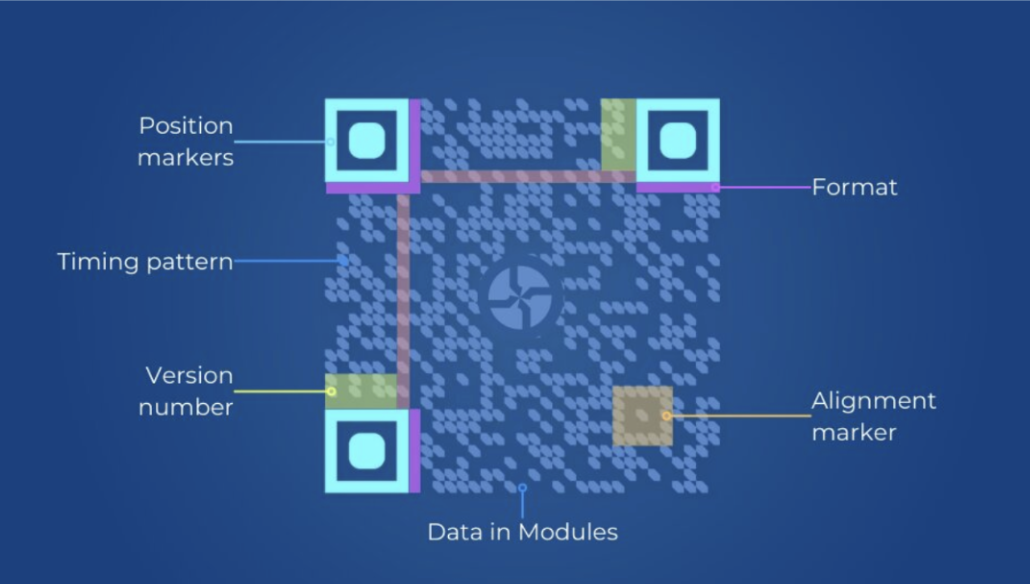
\includegraphics[width=\textwidth]{images/qr-structure.png}
        \\[2pt]
        {\scriptsize QR code structure \cite{uniqode2025}.}
      \end{center}
  \end{columns}
\end{frame}

\begin{frame}
  \frametitle{Three Pillars of QR Vulnerability}
  Despite ubiquity, standard QR payments exhibit \HL{three structural flaws}:
  \vspace{0.2cm}
  \begin{enumerate}
      \item \textbf{Physical / digital exploitation.} Cloning, ``\con{quishing}'' (QR phishing), and module-level overlays redirect users to phishing endpoints \cite{averin2020, canada2024, yong2019}.
      \item \textbf{Single point of failure (SPOF).} Existing joint-account systems sign with one central key. If compromised, the entire fund is lost.
      \item \textbf{Authentication dependency.} 2D barcodes carry no inherent cryptographic proof; defenses rely on post-scan backend validation, adding latency and risk.
  \end{enumerate}
\end{frame}

\begin{frame}
  \frametitle{Quishing in Action}
  \begin{columns}[T]
    \column{0.50\textwidth}
      \begin{itemize}
        \item Attacker alters a few modules of a benign QR with a pen or sticker.
        \item Encoded URL silently rewritten to a malicious target \cite{yong2019}.
        \item Email-distributed variant is the rising ``quishing'' vector \cite{canada2024}.
        \item Reed--Solomon error correction \cite{reed1960, bajaj2024} actually \con{helps} the attacker -- partial mutation still decodes.
      \end{itemize}
    \column{0.45\textwidth}
      \begin{center}
        
\includegraphics[width=\textwidth]{images/quishing.png}
        \\[2pt]
        {\scriptsize Module-level QR rewrite \cite{yong2019}.}
      \end{center}
  \end{columns}
\end{frame}

\begin{frame}
  \frametitle{Why Existing Mitigations Fall Short}
  \begin{center}
  \small
  \begin{tabular}{|p{0.27\textwidth}|p{0.30\textwidth}|p{0.30\textwidth}|}
    \hline
    \textbf{Approach} & \textbf{Strength} & \textbf{Gap} \\\hline
    Visual cryptography / steganography \cite{bhardwaj2024, ibrahim2021, narayanan2024} & Hides QR data / shares & Image stacking; still \con{single key} \\\hline
    ML-based scanners (QsecR, AP3X) \cite{rafsanjani2023, tayachi2025, rivas2025} & Detects malicious URLs $93$--$96\%$ & \con{Reactive}; no cryptographic proof \\\hline
    Dynamic QR (SQRC, UniQR) \cite{saranya2016, garnaik2022, wei2024} & Replay-resistant via freshness & Still \con{single signing key} \\\hline
  \end{tabular}
  \end{center}
  \vspace{0.15cm}
  \HL{None solves SPOF.} None binds multi-party consent into the QR itself.
\end{frame}

\begin{frame}
  \frametitle{Research Question}
  \begin{block}{Question}
    Can a \HL{$(t,n)$ threshold-signature protocol} secure joint-account QR payments \textit{without} sacrificing the latency users expect from mobile payments?
  \end{block}
  \vspace{0.2cm}
  \textbf{Sub-goals:}
  \begin{itemize}
      \item Eliminate SPOF via distributed key shares.
      \item Embed compact, verifiable authorisation \textit{into} the dynamic QR payload.
      \item Maintain $<200$ ms verification latency on commodity hardware.
      \item Validate functionality, security, and usability empirically.
  \end{itemize}
\end{frame}

% =====================================================================
\section{The What: Proposed Solution}
% =====================================================================

\begin{frame}
  \frametitle{Solution: Hybrid Threshold Cryptography}
  We synthesise three strands of the literature into one protocol:
  \vspace{0.2cm}
  \begin{enumerate}
      \item \textbf{Distributed trust.} Private key split into $n$ shares via DKG. Full key \HL{never reconstructed} -- forward secrecy \cite{shamir1979, ruffing2014}.
      \item \textbf{Multi-party approval.} Transactions need a quorum of $t$ members signing with distinct shares \cite{desmedt1988, gennaro2007}.
      \item \textbf{Dynamic freshness.} Nonces + timestamps cryptographically bound to the payload defeat replay \cite{boneh2001}.
  \end{enumerate}
  \vspace{0.2cm}
  \begin{block}{Threshold policy}
    Amount $< $ Php\,$1{,}000 \Rightarrow t = 1$ (instant). \\
    Amount $\ge $ Php\,$1{,}000 \Rightarrow t \ge 2$ (multi-party).
  \end{block}
\end{frame}

\begin{frame}
  \frametitle{Why ECC + BLS12-381 (and not RSA)?}
  \begin{columns}[T]
    \column{0.48\textwidth}
      \textbf{Stacked RSA / classical signatures}
      \begin{itemize}
        \item Each signer appends a 256-byte signature.
        \item QR payload grows \con{linearly} in $t$.
        \item Denser modules $\Rightarrow$ slower autofocus \cite{corpuz2025}.
        \item Verifier checks each independently.
      \end{itemize}
    \column{0.48\textwidth}
      \textbf{BLS12-381 threshold (ours)}
      \begin{itemize}
        \item All partial sigs aggregate into a \HL{single 48-byte $G_1$ element}.
        \item Payload size \HL{invariant in $t$}.
        \item One pairing equation verifies the quorum \cite{boneh2001}.
        \item Pairing-friendly curve at 128-bit security.
      \end{itemize}
  \end{columns}
  \vspace{0.15cm}
  \textit{BLS aggregation = same security, fewer bytes, faster scan.}
\end{frame}

\begin{frame}
  \frametitle{Why Distributed Key Generation?}
  Conventional dynamic-QR systems mint one secret and split or copy it. This \con{re-creates SPOF}.
  \vspace{0.2cm}
  \begin{itemize}
    \item \textbf{DKG:} the $n$ shares are generated jointly without ever materialising the full secret \cite{gennaro2007}.
    \item Each member's share $k_i$ lives only on their device.
    \item The joint public key $PK$ is derived as
      \[
      PK \;=\; \sum_{i=1}^{n} \lambda_i \cdot k_i \cdot g
      \]
    \item No single device, server, or moment in time holds the full key.
    \item Forward secrecy \HL{by construction} -- compromise of $< t$ shares leaks nothing.
  \end{itemize}
\end{frame}

\begin{frame}
  \frametitle{Cryptographic Core: Partial Signing}
  Each approving member computes a partial signature on the SHA-256 digest of the transaction message $M = \{\textit{Merchant\_ID}, \textit{Amount}, \textit{Timestamp}, \textit{Nonce}\}$:
  \[
  \sigma_i \;=\; H(M)^{k_i} \;=\; k_i \cdot H(M)
  \]
  The Payer aggregates any valid $t$ partials via Lagrange interpolation:
  \[
  F_{\text{sig}} \;=\; \sum_{i=1}^{t} \lambda_i \cdot \sigma_i \;=\; \sum_{i=1}^{t} \lambda_i \cdot k_i \cdot H(M)
  \]
  \vspace{-0.15cm}
  \begin{itemize}
    \item Output is mathematically equivalent to signing with the full key.
    \item Full key is \HL{never reconstructed} at any party \cite{shamir1979, komlo2021}.
  \end{itemize}
\end{frame}

\begin{frame}
  \frametitle{Verification: Bilinear Pairing}
  The Verifier (Merchant) checks one pairing equation \cite{john2023}:
  \[
  e(F_{\text{sig}},\, g) \;\stackrel{?}{=}\; e(H(M),\, PK)
  \]
  Bilinearity ($e(aP, bQ) = e(P,Q)^{ab}$) makes both sides equal:
  \[
  \prod_{i=1}^{t} e(H(M), g)^{\lambda_i \cdot k_i}
  \]
  \vspace{-0.2cm}
  \begin{itemize}
    \item Verifier \HL{never sees} any private share.
    \item Verifier holds only the public $PK$ -- no coordination state.
    \item Pairing in constant time regardless of $t$.
  \end{itemize}
\end{frame}

\begin{frame}
  \frametitle{End-to-End Protocol Flow}
  \begin{center}
    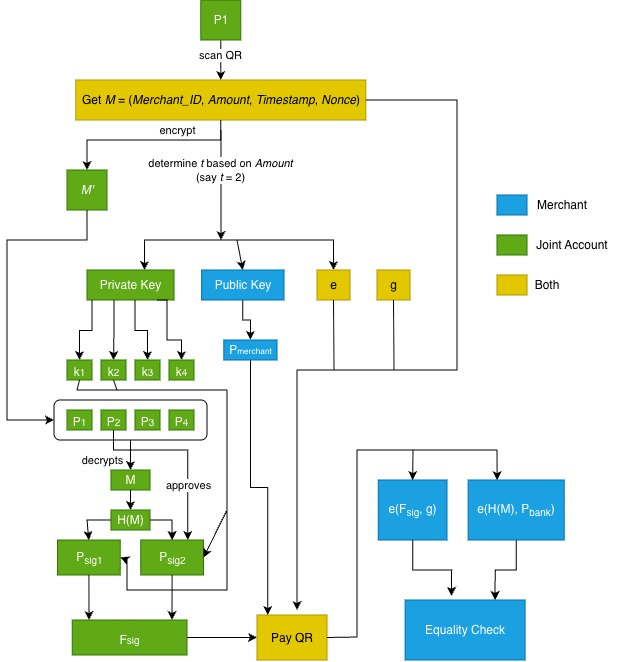
\includegraphics[width=0.78\textwidth, height=0.65\textheight, keepaspectratio]{images/method_diag.png}
  \end{center}
  \vspace{-0.1cm}
  {\scriptsize Five phases: Initiation $\rightarrow$ Policy/threshold $\rightarrow$ Key share retrieval $\rightarrow$ Distributed signing \& aggregation $\rightarrow$ Dynamic QR \& verification.}
\end{frame}

% =====================================================================
\section{The How: System Architecture}
% =====================================================================

\begin{frame}
  \frametitle{Technology Stack: Justification}
  \begin{center}
  \small
  \begin{tabular}{|p{0.22\textwidth}|p{0.22\textwidth}|p{0.45\textwidth}|}
    \hline
    \textbf{Layer} & \textbf{Choice} & \textbf{Why} \\\hline
    Frontend & React 18 + Vite & Component model fits role-based dashboards; Vite HMR for rapid iteration; native socket integration. \\\hline
    Real-time & Socket.io / WebSockets & Threshold signing is \HL{event-driven}; REST polling would inflate latency and miss approvals. \\\hline
    Persistence & MongoDB 6+ (NoSQL) & Document model = single-write transaction state; fast reads vs. relational joins; matches our 6-state machine. \\\hline
    Crypto & \texttt{@noble/curves} (pure JS) & Audited BLS12-381 primitives; portable client \emph{and} server; no native build step. \\\hline
  \end{tabular}
  \end{center}
\end{frame}

\begin{frame}
  \frametitle{Architecture: Honest-but-Curious Proxy}
  \begin{itemize}
      \item \textbf{Three roles:} \pos{Initiator} (Buyer), \pos{Approver} (Buyer), \pos{Verifier} (Merchant). Each maps to a Socket.io room.
      \item \textbf{Proxy server} relays AES-256-GCM encrypted partial shares between members.
      \item Ephemeral Diffie--Hellman session keys $\Rightarrow$ proxy sees \HL{only ciphertext} \cite{chen2011, ruffing2014}.
      \item \textbf{Lock map} (\texttt{transactionLocks}) serialises concurrent \texttt{submit\_share} on the same transaction -- defeats race-based double-spend.
      \item \textbf{Audit log:} 12 event types broadcast to all clients in real time.
  \end{itemize}
\end{frame}

\begin{frame}
  \frametitle{Transaction State Machine}
  \begin{center}
    \small
    \texttt{PENDING} $\rightarrow$ \texttt{COMPLETING} $\rightarrow$ \texttt{COMPLETED} $\rightarrow$ \texttt{PAID} \\[4pt]
    {\scriptsize Branches: $\rightarrow$ \texttt{EXPIRED} (2-min QR TTL) \quad $\rightarrow$ \texttt{CANCELLED} / \texttt{FAILED}}
  \end{center}
  \vspace{0.15cm}
  \begin{itemize}
    \item Background sweeper checks expiry every 10 s.
    \item Authoritative \texttt{Amount} read from the persisted document at verification -- never from the client envelope (see Phase 2b).
    \item State transitions emit \texttt{transaction\_completed}, \texttt{balance\_update}, and \texttt{occupied\_nodes\_update} broadcasts.
  \end{itemize}
\end{frame}

\begin{frame}
  \frametitle{Five-Phase Validation Pipeline}
  Design-Science framework: \HL{inside-out validation}.
  \vspace{0.2cm}
  \begin{enumerate}
      \item \textbf{Phase 1 -- Cryptographic unit testing.} Isolate BLS12-381 primitives; prove correctness.
      \item \textbf{Phase 2 -- Pentest \& benchmarks.} Adversarial scenarios + latency profile.
      \item \textbf{Phase 3 -- UAT Cycle 1.} Formative usability (5 participants).
      \item \textbf{Phase 4 -- UI refinement.} Targeted fixes from Cycle 1.
      \item \textbf{Phase 5 -- UAT Cycle 2.} Final baseline (10 participants, 2 groups).
  \end{enumerate}
  \vspace{0.1cm}
  \textit{Ordering matters: never test usability on broken crypto, never claim security on un-benchmarked code.}
\end{frame}

% =====================================================================
\section{Results: Cryptography \& Performance}
% =====================================================================

\begin{frame}
  \frametitle{Phase 1: Cryptographic Correctness (35/35)}
  \begin{center}
  \small
  \begin{tabular}{|c|l|c|c|}
    \hline
    \# & Category & Tests & Result \\\hline
    1 & Hash function (\texttt{hashMessage}) & 5 & 5/5 \\\hline
    2 & Partial signing (\texttt{signMessage}) & 5 & 5/5 \\\hline
    3 & Threshold configuration & 6 & 6/6 \\\hline
    4 & All ten 3-of-5 combinations & 10 & 10/10 \\\hline
    5 & Insufficient signers (sub-threshold) & 2 & 2/2 \\\hline
    6 & Tamper-resistance (payload attacks) & 6 & 6/6 \\\hline
    7 & Aggregation error handling & 1 & 1/1 \\\hline
    \multicolumn{2}{|r|}{\textbf{Total}} & \textbf{35} & \textbf{35/35} \\\hline
  \end{tabular}
  \end{center}
  \vspace{0.15cm}
  Completed in \HL{707 ms} on the dev machine. Every 2-of-5 sub-threshold attempt failed pairing -- the formal expression of threshold security.
\end{frame}

\begin{frame}
  \frametitle{Phase 2a: Verification Latency (n=30)}
  \begin{columns}[T]
    \column{0.50\textwidth}
      \small
      \begin{tabular}{|l|c|c|}
        \hline
        Metric & QR Gen & Verify \\\hline
        Min & 19 ms & 3 ms \\\hline
        Max & 32 ms & 8 ms \\\hline
        \HL{Mean} & 24.73 ms & \HL{4.83 ms} \\\hline
        Std dev & 2.87 ms & 1.21 ms \\\hline
        p50 & 24 ms & 5 ms \\\hline
        p95 & 31 ms & 7 ms \\\hline
        \HL{p99} & 32 ms & \HL{8 ms} \\\hline
      \end{tabular}
    \column{0.45\textwidth}
      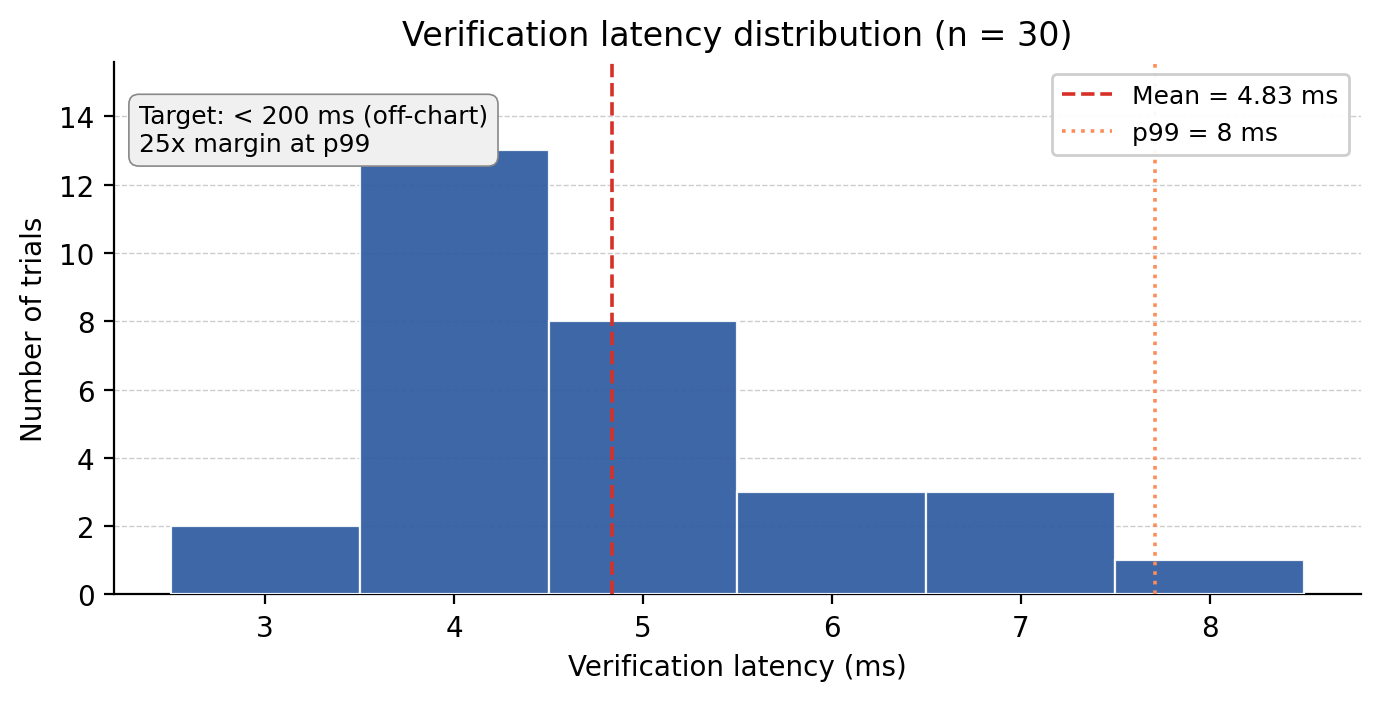
\includegraphics[width=\textwidth]{images/fig_latency.png}
  \end{columns}
  \vspace{0.15cm}
  Acceptance criterion: verification $< 200$ ms. \\
  \HL{Result: 30/30 PASS}, with $25\times$ margin at p99.
\end{frame}

\begin{frame}
  \frametitle{Why Latency Headroom Matters}
  \begin{itemize}
      \item BLS aggregates $t$ partials into a \HL{single $G_1$ element} -- post-aggregation QR size is invariant in $t$.
      \item Verifier work is one pairing + one Mongo \texttt{findOne} + one \texttt{save}.
      \item Production deployment adds $50$--$150$ ms geographic routing -- still well below 200 ms.
      \item Room to add zero-knowledge attestations, freshness proofs, etc., without breaching the criterion.
  \end{itemize}
  \vspace{0.1cm}
  \begin{block}{Bottom line}
    Performance budget is \HL{comfortably absorbing}, not pinched.
  \end{block}
\end{frame}

\begin{frame}
  \frametitle{Phase 2b: Adversarial / MITM Validation (13/13)}
  \begin{center}
  \scriptsize
  \begin{tabular}{|c|l|c|}
    \hline
    \# & Scenario & Outcome \\\hline
    A1 & BLS forgery: random bytes as signature & \pos{Blocked} \\\hline
    A2 & BLS forgery: all-zero signature bytes & \pos{Blocked} \\\hline
    A3 & Amount tampering on a valid signature & \pos{Blocked} \\\hline
    A4 & Nonce replacement on a valid signature & \pos{Blocked} \\\hline
    A5 & Cross-transaction signature reuse & \pos{Blocked} \\\hline
    A6 & 2-of-5 threshold attack & \pos{Blocked} \\\hline
    A7 & Positive control (legit 3-of-5 sig) & \pos{Accepted} \\\hline
    B1 & \texttt{verify\_payment} with nonexistent nonce & \pos{Blocked} \\\hline
    B2 & Amount inflation (Php 999{,}999 vs.\ stored Php 100) & \pos{Blocked} \\\hline
    B3 & Amount deflation (Php 1 vs.\ stored Php 500) & \pos{Blocked} \\\hline
    B4 & Positive control (legit verify) & \pos{Accepted} \\\hline
    B5 & Replay of a \texttt{PAID} transaction & \pos{Blocked} \\\hline
    B6 & Premature verify (\texttt{PENDING} transaction) & \pos{Blocked} \\\hline
  \end{tabular}
  \end{center}
\end{frame}

\begin{frame}
  \frametitle{Operational Vulnerability Found \& Patched}
  \textbf{B2 and B3 are not cryptographic tests} -- they exercise the application logic.
  \vspace{0.15cm}
  \begin{block}{The bug (pre-patch)}
    \texttt{socketHandler.js} deducted \texttt{data.amount} -- the \HL{client-supplied} value -- even when the signature was bound to a different amount.
  \end{block}
  \vspace{0.1cm}
  \begin{itemize}
    \item A TLS-breaking adversary could swap Php 100 $\rightarrow$ Php 999{,}999 \textit{after} signing.
    \item BLS math was correct. Application logic was not.
  \end{itemize}
  \begin{block}{The patch}
    Server reads the authoritative \texttt{Amount} from the persisted \texttt{Transaction} document, ignoring the client field.
  \end{block}
  \HL{Takeaway:} A secure protocol still needs disciplined application logic around it.
\end{frame}

\begin{frame}
  \frametitle{Sample MITM Test Output}
\begin{lstlisting}
-- OFFLINE CRYPTOGRAPHIC INTEGRITY TESTS --
 [BLOCKED] BLS forgery: random bytes as signature
        Server: "Pairing mismatch -- rejected"
 [BLOCKED] BLS tamper: valid sig, amount changed to Php 1
        Server: "Hash mismatch -- rejected"
 [BLOCKED] Threshold attack: 2-of-5 shares as full signature
        Server: "Lagrange reconstruction fails -- rejected"

-- ONLINE PROTOCOL ATTACK TESTS --
 [BLOCKED] Protocol: amount inflation (socket Php 999,999 vs stored Php 100)
        Server: "Deducted Php 100 = stored Php 100 (BLOCKED)"
 [BLOCKED] Protocol: replay attack -- re-verify an already-PAID transaction
\end{lstlisting}
  \vspace{0.05cm}
  \HL{All 13 scenarios resolve as expected}; failures are \textit{fail-closed} (no oracle leak).
\end{frame}

% =====================================================================
\section{Results: Usability \& Iteration}
% =====================================================================

\begin{frame}
  \frametitle{Phase 3: UAT Cycle 1 -- Friction Surfaced}
  Five participants, ten task scenarios, role-rotated (Shopper / Approver / Cashier).
  \vspace{0.15cm}
  \begin{itemize}
      \item \textbf{Scenario coverage: 10/10 PASS} -- including race conditions, double-scan prevention, and the 2-min QR-expiry case.
      \item \textbf{The signal was not a failure -- it was the open-ended feedback.}
      \item \HL{4 of 5} participants asked for a visible countdown of remaining QR validity (``timer for expiring QR code'', ``more explicit timers (graphic or numerical)'').
  \end{itemize}
  \vspace{0.15cm}
  \begin{block}{Diagnosis}
    Dominant friction is \HL{temporal-perceptual}, not cryptographic. Backend resolves in ${<}30$ ms; user feels a 2-minute window with no cue.
  \end{block}
\end{frame}

\begin{frame}
  \frametitle{Phase 4: Two Refinements}
  Decision rule: refinements may touch interaction and encoding layers \textit{only} -- never the crypto, message format, or threshold policy. Otherwise Phase 1/2 evidence is invalidated.
  \vspace{0.15cm}
  \begin{enumerate}
    \item \textbf{Visible countdown timer.} Renders \texttt{qrExpiresAt} continuously on the Shopper's screen. Purely presentational.
    \item \textbf{Small QR encoding (new variant).} QR carries a \HL{short reference token} (${\sim}21$ bytes) instead of the full $\{PK, g, F_{\text{sig}}, M\}$ envelope (${\sim}443$ bytes). Verifier fetches the envelope out-of-band over the existing trusted channel.
  \end{enumerate}
  \vspace{0.1cm}
  \textit{Both refinements re-ran Phase 1 + Phase 2 -- all tests still pass.}
\end{frame}

\begin{frame}
  \frametitle{Big QR vs Small QR}
  \begin{columns}[T]
    \column{0.50\textwidth}
      \begin{center}
        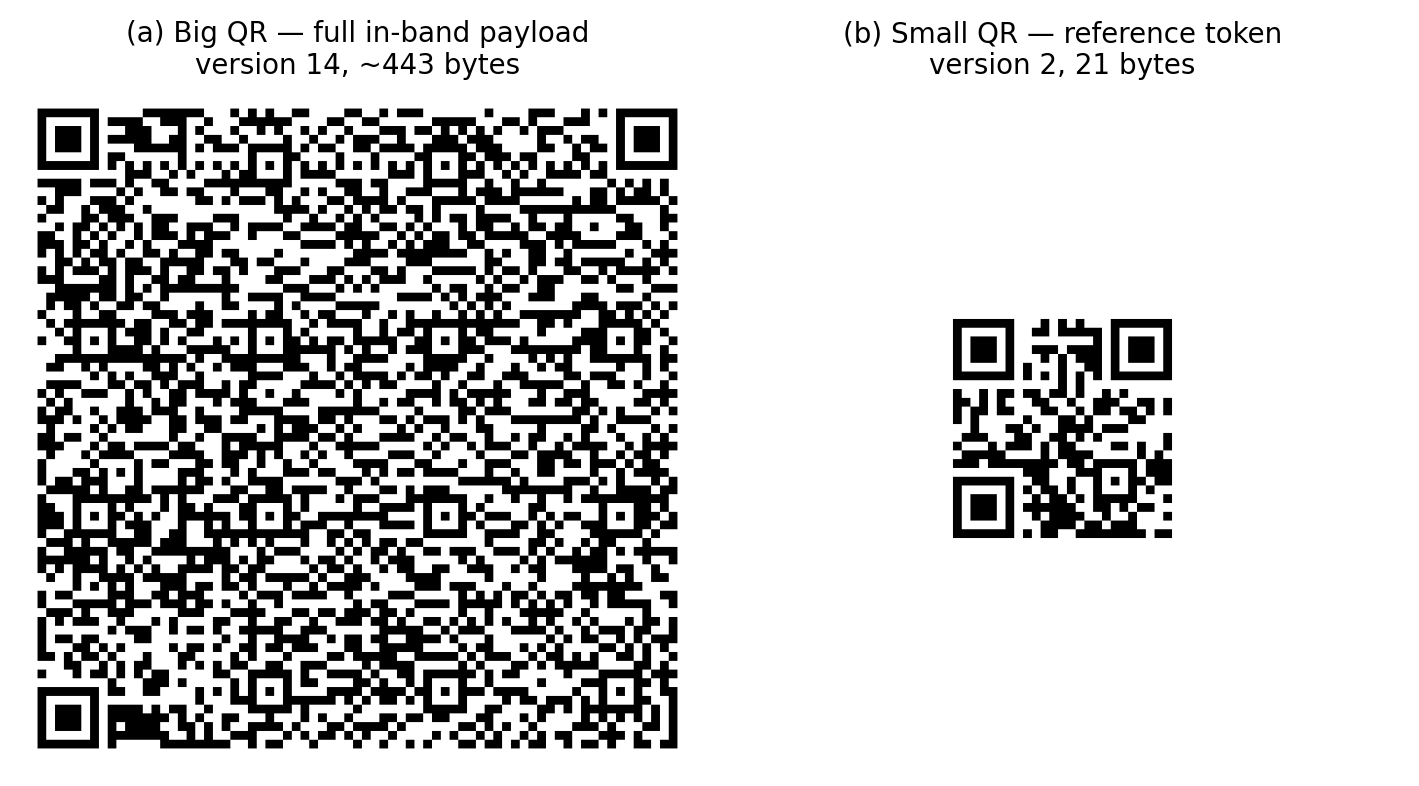
\includegraphics[width=0.95\textwidth]{images/fig_qr_comparison.png}
      \end{center}
    \column{0.45\textwidth}
      \textbf{Big QR (in-band):}
      \begin{itemize}
        \item \pos{Self-contained} cryptographic proof.
        \item \con{Dense modules} $\Rightarrow$ slower autofocus.
      \end{itemize}
      \textbf{Small QR (out-of-band):}
      \begin{itemize}
        \item \pos{Sparser grid}, instant scan.
        \item \con{Shifts trust} to the TLS retrieval channel.
      \end{itemize}
  \end{columns}
\end{frame}

\begin{frame}
  \frametitle{Phase 5: UAT Cycle 2 -- SUS Scores (n=10)}
  \begin{center}
  \small
  \begin{tabular}{|l|l|c|}
    \hline
    Group & Participant & $\textit{SUS}_{6}$ \\\hline
    A (Big QR)   & P1, P2, P3, P4, P5 & 91.7, 100, 91.7, 91.7, 100 \\\hline
    \multicolumn{2}{|r|}{\textbf{Group A mean}} & \textbf{95.0} \\\hline
    B (Small QR) & P6, P7, P8, P9, P10 & 79.2, 58.3, 79.2, 33.3, 54.2 \\\hline
    \multicolumn{2}{|r|}{\textbf{Group B mean}} & \textbf{60.8} \\\hline
    \multicolumn{2}{|r|}{\textbf{Overall ($n=10$)}} & \HL{\textbf{77.9}} \\\hline
  \end{tabular}
  \end{center}
  \vspace{0.15cm}
  \begin{itemize}
    \item Aggregate \HL{77.9} sits above the $68$-point conventional acceptability threshold \cite{brooke1996sus, bangor2008sus}.
    \item Group B lower mean driven by \textbf{two} participants pairing low ratings with substantive design critiques -- \HL{not} a scannability penalty (see next slide).
  \end{itemize}
\end{frame}

\begin{frame}
  \frametitle{QR Scannability (Item 4.2)}
  \begin{columns}[T]
    \column{0.48\textwidth}
      \begin{center}
        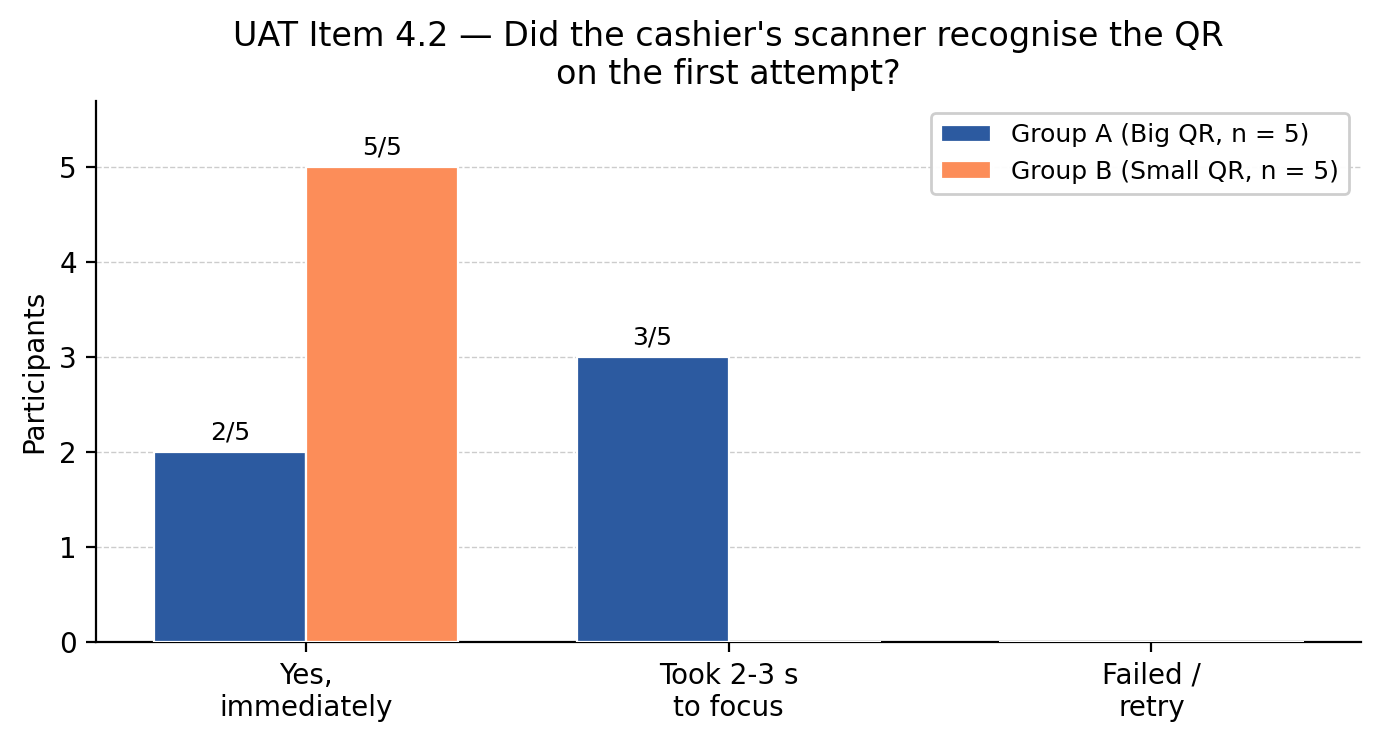
\includegraphics[width=\textwidth]{images/fig_qr_recognition.png}
      \end{center}
    \column{0.50\textwidth}
      \small
      \begin{tabular}{|l|c|c|}
        \hline
        Response & Big QR & Small QR \\\hline
        Yes, immediately & 4/5 & \HL{5/5} \\\hline
        2--3 s focus delay & 1/5 & 0/5 \\\hline
        Failed / retry & 0/5 & 0/5 \\\hline
      \end{tabular}
      \vspace{0.2cm}
      \begin{itemize}
        \item Direction matches the QR module-density effect \cite{corpuz2025}.
        \item No \textit{hard} scan failure in either group.
        \item Reported as modest, direction-only signal -- not a point estimate.
      \end{itemize}
  \end{columns}
\end{frame}

\begin{frame}
  \frametitle{Perceived Security \& Open-Ended Feedback}
  \textbf{Item 5.1 -- Multi-party approval makes you feel safer?}
  \begin{itemize}
      \item \HL{10/10} Cycle-2 participants: ``Yes, significantly'' (7) or ``Somewhat safer'' (3).
      \item Zero ``No difference''. Zero ``Felt less secure''.
      \item Consistent with \cite{komlo2021, krombholz2014}: \textit{procedural friction dominates} perceived security over invisible cryptography.
  \end{itemize}
  \vspace{0.15cm}
  \textbf{Four open-ended themes (drive Section 6 recommendations):}
  \begin{enumerate}
      \item \textbf{Deposit feature} (4/5 Big QR participants).
      \item \textbf{Stricter credential confirmation} -- biometrics, PIN, OTP (3 participants).
      \item \textbf{Push notifications} for pending approvals (2 participants).
      \item \textbf{Sub-threshold splitting} loophole (1 participant -- correct critique).
  \end{enumerate}
\end{frame}

% =====================================================================
\section{Discussion}
% =====================================================================

\begin{frame}
  \frametitle{Cryptographic vs.\ Operational Security}
  \begin{itemize}
      \item BLS guarantees are \HL{unconditional} -- they follow from EC-DLP hardness.
      \item Application-level guarantees depend on \HL{disciplined software}.
      \item B2/B3 amount-tampering attack: math was perfect, but the server trusted the client's \texttt{amount} field.
  \end{itemize}
  \vspace{0.15cm}
  \begin{block}{Lesson}
    A mathematically secure threshold signature is \HL{necessary but not sufficient}. Application logic must actively protect the fields that the signature binds.
  \end{block}
  \vspace{0.1cm}
  Regression tests B2 and B3 now lock down the patched behaviour.
\end{frame}

\begin{frame}
  \frametitle{Latency Headroom vs.\ Felt Latency}
  \begin{itemize}
      \item \textbf{Mean verification 4.83 ms} -- 25$\times$ margin against the 200 ms target.
      \item Room to add zero-knowledge proofs, freshness attestations, etc.
      \item But \HL{users do not perceive backend round-trip speed}.
      \item User experience is dominated by:
        \begin{itemize}
          \item The 2-minute QR-expiry countdown (Phase 4 fix).
          \item Camera autofocus on dense QR (Big QR vs Small QR).
        \end{itemize}
  \end{itemize}
  \vspace{0.15cm}
  \HL{Felt latency} is a psychological budget -- not a computational one.
\end{frame}

\begin{frame}
  \frametitle{The QR Scannability Trade-off}
  \begin{center}
  \small
  \begin{tabular}{|p{0.18\textwidth}|p{0.32\textwidth}|p{0.32\textwidth}|}
    \hline
    & \textbf{Big QR (in-band)} & \textbf{Small QR (out-of-band)} \\\hline
    Self-contained & \pos{Yes -- offline verifiable} & \con{No -- needs fetch} \\\hline
    Module density & \con{High} & \pos{Low} \\\hline
    Scan speed (UAT) & 4/5 immediate & \pos{5/5 immediate} \\\hline
    Trust surface & \pos{Cryptographic content only} & \con{+ TLS retrieval channel} \\\hline
  \end{tabular}
  \end{center}
  \vspace{0.15cm}
  \HL{Recommendation:} make encoding a per-transaction Policy Engine decision keyed by value.
\end{frame}

\begin{frame}
  \frametitle{Limitations}
  \begin{enumerate}
      \item \textbf{Sample size.} 15 total UAT participants; six-item SUS adaptation departs from the canonical instrument.
      \item \textbf{Localhost benchmarks.} Network RTT added qualitatively, not measured on the production cloud path.
      \item \textbf{Threat model boundary.} MITM scope = network adversary; \HL{endpoint compromise} (stolen unlocked phone, $t$ compromised devices) is out of scope.
      \item \textbf{Sub-threshold splitting.} Memoryless threshold policy: $50 \times $ Php $999$ transactions individually authorise at $t=1$ -- a malicious co-owner can drain a balance.
  \end{enumerate}
\end{frame}

% =====================================================================
\section{Recommendations \& Conclusion}
% =====================================================================

\begin{frame}
  \frametitle{Recommendations: Policy \& Thresholding}
  \begin{enumerate}
      \item \textbf{Adaptive QR sizing by risk.} Policy Engine picks Small QR for low-risk (UX-first) and Big QR for high-value (offline-security-first) \cite{corpuz2025, reed1960, bajaj2024}.
      \item \textbf{Joint fund replenishment.} Symmetric thresholding on deposits, with an explicit \textit{source-of-funds} field. Non-suppressible audit event regardless of threshold.
      \item \textbf{Velocity limits on sub-threshold payments.} Rolling 24-hour total of $t{=}1$ debits per member. Crossing the Php 1{,}000 quorum trigger \HL{escalates} subsequent transactions to $t \ge 2$ until the window rolls over.
  \end{enumerate}
\end{frame}

\begin{frame}
  \frametitle{Recommendations: Authentication \& UX}
  \begin{enumerate}
      \setcounter{enumi}{3}
      \item \textbf{Multi-factor approval confirmation.} Bind each \texttt{submit\_share} to a fresh \HL{local biometric / PIN / hardware-token} check. Possession of an unlocked phone $\neq$ consent.
      \item \textbf{Out-of-band notifications.} APNs / FCM push for pending approvals carry only an opaque session ID -- preserves the proxy's honest-but-curious trust boundary.
  \end{enumerate}
\end{frame}

\begin{frame}
  \frametitle{Recommendations: Long-Term Architecture}
  \begin{enumerate}
      \setcounter{enumi}{5}
      \item \textbf{Proactive secret sharing.} Periodic share refresh (without changing $PK$) defeats long-term endpoint compromise \cite{shamir1979, gennaro2007, komlo2021}.
      \item \textbf{Hardware-backed key storage.} Move shares into Secure Enclave (Apple) / StrongBox (Android). Partial signing as an opaque service.
      \item \textbf{Post-quantum migration.} Keep $F_{\text{sig}}$ as an opaque blob behind a primitive-agnostic verification interface; swap BLS for a lattice-based threshold variant when ready.
  \end{enumerate}
\end{frame}

\begin{frame}
  \frametitle{Conclusion}
  A $(t,n)$ threshold-signature protocol on BLS12-381 delivers \HL{robust, decentralised} security for joint-account QR payments \HL{without sacrificing mobile latency}.
  \vspace{0.2cm}
  \begin{itemize}
      \item \pos{SPOF eliminated} -- distributed trust by construction (DKG).
      \item \pos{Lightning fast} -- mean verification $4.83$ ms, $25\times$ margin at p99.
      \item \pos{Adversarially resilient} -- 13/13 attack scenarios resolved as expected.
      \item \pos{User validated} -- aggregate SUS $77.9$, 10/10 perceived-safety positive.
      \item \pos{Reproducible} -- 35/35 unit tests, two-cycle UAT, public deployment.
  \end{itemize}
  \vspace{0.15cm}
  \textit{Threshold cryptography is no longer just theoretical -- it is a practical primitive for joint-account payment systems.}
\end{frame}

% =====================================================================
\section*{References}
% =====================================================================

\begin{frame}[allowframebreaks]
  \frametitle{References}
  \scriptsize
  \begin{thebibliography}{99}
    \bibitem{tu2022} M.~Tu \emph{et~al.}, ``The adoption of QR code mobile payment technology during COVID-19,'' \emph{Frontiers in Psychology}, vol.~12, 2022.
    \bibitem{sonowal2024} G.~Sonowal, ``QR Code Phishing: A Review of the Current Attacks and Countermeasures,'' \emph{Juni Khyat Journal}, 2024.
    \bibitem{averin2020} A.~Averin and N.~Zyulyarkina, ``Malicious QR-Code Threats and Vulnerability of Blockchain,'' \emph{GloSIC}, 2020.
    \bibitem{yong2019} K.~S.~C.~Yong, K.~L.~Chiew and C.~L.~Tan, ``A Survey of the QR Code Phishing,'' \emph{ICSCC}, 2019.
    \bibitem{canada2024} Canadian Centre for Cyber Security, ``Security Considerations for QR Codes (ITSAP.00.141),'' 2024.
    \bibitem{krombholz2014} K.~Krombholz \emph{et~al.}, ``QR Code Security: A Survey of Attacks and Challenges for Usable Security,'' Springer, 2014.
    \bibitem{corpuz2025} D.~J.~Corpuz \emph{et~al.}, ``QR code detection with perspective correction and decoding in real-world conditions,'' \emph{VISAPP}, 2025.
    \bibitem{worldbank2021} The World Bank, ``The use of quick-response codes in payments -- Ch.~2,'' 2021.
    \bibitem{worldbank2021ch5} The World Bank, ``The use of quick-response codes in payments -- Ch.~5,'' 2021.
    \bibitem{sankara2012} N.~Sankara, ``QR codes and security solutions,'' \emph{IJCST}, vol.~3, no.~7, 2012.
    \bibitem{uniqode2025} Uniqode, ``The Ultimate Guide to QR Codes,'' 2025.
    \bibitem{reed1960} I.~Reed and G.~Solomon, ``Polynomial Codes Over Certain Finite Fields,'' \emph{SIAM J.}, vol.~8, no.~2, 1960.
    \bibitem{bajaj2024} B.~S.~Bajaj, ``Reliability on QR Codes and Reed-Solomon codes,'' 2024.
    \bibitem{bhardwaj2024} N.~Bhardwaj \emph{et~al.}, ``Visual cryptography and steganography in QR codes,'' 2024.
    \bibitem{ibrahim2021} D.~R.~Ibrahim \emph{et~al.}, ``Visual cryptography for QR codes,'' 2021.
    \bibitem{narayanan2024} S.~Narayanan \emph{et~al.}, ``LFSR / Rubik's cube AES on QR codes,'' 2024.
    \bibitem{rafsanjani2023} A.~Rafsanjani \emph{et~al.}, ``QsecR: secure Android QR scanner,'' 2023.
    \bibitem{tayachi2025} N.~Tayachi \emph{et~al.}, ``ML for malicious QR URL detection,'' 2025.
    \bibitem{rivas2025} L.~Rivas \emph{et~al.}, ``AP3X Secure QR Codes Infrastructure,'' 2025.
    \bibitem{saranya2016} K.~Saranya \emph{et~al.}, ``Secured QR Code (SQRC),'' 2016.
    \bibitem{garnaik2022} S.~Garnaik and J.~Ryoo, ``Rotation-based dynamic QR payments,'' 2022.
    \bibitem{wei2024} C.~Wei \emph{et~al.}, ``UniQR: pose-bound QR codes,'' 2024.
    \bibitem{shamir1979} A.~Shamir, ``How to share a secret,'' \emph{Comm.~ACM}, vol.~22, no.~11, 1979.
    \bibitem{desmedt1988} Y.~Desmedt, ``Society and group oriented cryptography,'' \emph{CRYPTO}, 1988.
    \bibitem{gennaro2007} R.~Gennaro \emph{et~al.}, ``Secure Distributed Key Generation for Discrete-Log Based Cryptosystems,'' \emph{J.~Cryptology}, 2007.
    \bibitem{boneh2001} D.~Boneh, B.~Lynn, H.~Shacham, ``Short Signatures from the Weil Pairing,'' \emph{ASIACRYPT}, 2001.
    \bibitem{chen2011} L.~Chen \emph{et~al.}, ``Proxy re-encryption,'' 2011.
    \bibitem{ruffing2014} T.~Ruffing \emph{et~al.}, ``CoinShuffle: practical decentralized coin mixing,'' \emph{ESORICS}, 2014.
    \bibitem{komlo2021} C.~Komlo and I.~Goldberg, ``FROST: Flexible Round-Optimized Schnorr Threshold Signatures,'' \emph{SAC}, 2021.
    \bibitem{john2023} J.~John, ``On bilinear pairings in elliptic curves,'' 2023.
    \bibitem{brooke1996sus} J.~Brooke, ``SUS: A quick and dirty usability scale,'' 1996.
    \bibitem{bangor2008sus} A.~Bangor, P.~T.~Kortum, J.~T.~Miller, ``An empirical evaluation of the System Usability Scale,'' \emph{IJHCI}, vol.~24, 2008.
  \end{thebibliography}
\end{frame}

\begin{frame}
  \begin{center}
    \Huge Thank You \\
    \vspace{0.5cm}
    \Large Questions?
  \end{center}
\end{frame}

% =====================================================================
\appendix
\section*{Backup Slides}
% =====================================================================

\begin{frame}
  \frametitle{Backup: BLS12-381 Field Constants}
  \begin{itemize}
    \item Curve: BLS12-381 via \texttt{@noble/curves}.
    \item Scalar field order:
      {\small \texttt{0x73eda753299d7d483339d80809a1d805} \\
              \texttt{53bda402fffe5bfeffffffff00000001}}
    \item Pairing target: $G_T \subset \mathbb{F}_{q^{12}}$.
    \item Compressed $G_1$ element: 48 bytes.
    \item BLS aggregate: one $G_1$ point regardless of $t$.
  \end{itemize}
\end{frame}

\begin{frame}
  \frametitle{Backup: Lagrange Coefficients}
  For signer set $S$ with $|S| = t$:
  \[
  \lambda_i \;=\; \prod_{j \in S,\, j \neq i} \frac{0 - j}{i - j}
  \]
  Reconstruction (at $x = 0$, never materialised on the wire):
  \[
  \text{secret} \;\equiv\; \sum_{i \in S} \lambda_i \cdot k_i \pmod{\text{ORDER}}
  \]
  In our prototype: $k_i = (\text{secret} + i + i^2) \bmod \text{ORDER}$ for $i \in \{1, \ldots, 5\}$.
\end{frame}

\begin{frame}
  \frametitle{Backup: Production Deployment}
  \begin{itemize}
    \item Backend: Render (\url{https://thesis-qr.onrender.com}). Node 18+, Express, Socket.io.
    \item Frontend: Vercel via \texttt{auto-deploy.yml} on push to \texttt{main}.
    \item Transport: WebSocket Secure (\texttt{wss://}) over TLS 1.3.
    \item Persistence: MongoDB Atlas; \texttt{Transaction}, \texttt{GroupBalance}, \texttt{AuditLog}.
    \item All MITM tests still pass under \HL{TLS-broken} threat model.
  \end{itemize}
\end{frame}

\begin{frame}
  \frametitle{Backup: Threat Model Boundary}
  \begin{center}
  \small
  \begin{tabular}{|p{0.36\textwidth}|c|}
    \hline
    \textbf{Scenario} & \textbf{In scope?} \\\hline
    Passive network eavesdropper & \pos{Yes} \\\hline
    TLS-breaking active MITM & \pos{Yes} \\\hline
    Compromised proxy (honest-but-curious) & \pos{Yes} \\\hline
    Single share leakage ($< t$) & \pos{Yes} (resists) \\\hline
    Coalition of $t$ compromised devices & \con{No -- by construction} \\\hline
    Stolen unlocked device & \con{No -- needs Rec.~4} \\\hline
    Quantum adversary & \con{No -- needs Rec.~8} \\\hline
  \end{tabular}
  \end{center}
\end{frame}

\end{document}
